\documentclass{article}
\usepackage{fullpage}
\usepackage[utf8]{inputenc}
\usepackage{graphicx}
\usepackage{hyperref}
\usepackage{tabularx}
\usepackage{attachfile}
\usepackage{caption} \captionsetup[table]{skip=10pt}

\title{Basic Lab Course 1: Pendulum (PEN)}
\author{Technical University of Munich\\\\Leon Heiß, Paul Hildebrandt \\
Course 5, Group 7, Team 19}
\date{31 May 2022}
\renewcommand*\contentsname{Contents}

\begin{document}

\maketitle
\large
\begin{center}
\textbf{Abstract}\\
\normalsize
\medskip

The objective of the pendulum experiment is to examine the behaviour of two different pendulum setups.
In the first part of the experiment a reversible pendulum is used to determine earth's gravitational acceleration. The second part deals with two methods of deflection to attain varying oscillations as well as the beating of a coupled pendulum.

\end{center}
\normalsize

\tableofcontents

\section{Reversed pendulum}
\subsection{Theory}
The most popular approach of discussing a simple pendulum is performed assuming all mass in one point.
This means neither may the connection between the mass and the hinge have any mass nor may the mass have any volume.
Obviously, this is not the case for the real world. For more accurate calculations, we need to update these assumptions.
Even while still disregarding friction, more accurate results can be achieved observing the pendulums moment of inertia using
\begin{equation}
g = 4\pi^2 \cdot \frac{J_c+m\cdot l^2}{m\cdot l \cdot \tau^2}
\end{equation} 
with the acceleration $g$, the moment of inertia $J_c$ from the center of mass, the mass $m$ and the length $l$ from the hinge to the center of mass \cite{1}.
But since a pendulum has a shape that differs from any perfect mathematical object and thereby the moment of inertia can not be calculated exactly, we can try to eliminate the moment of inertia from equation 1.
It appears that, for this quadratic equation, two different values for $l$, $l_1$ and $l_2$ exist, that result in the same value for $g$.
This can be interpreted as two different distances from the center of mass that result in the same period $\tau$.
We receive
\begin{equation}
g = 4 \pi^2 \cdot \frac{l_1 + l_2}{\tau^2}.
\end{equation}
$l_1 + l_2$ can be replaced by a constant distance $L$ for our experiment.
The resulting equation 
\begin{equation}
g = 4 \pi^2 \cdot \frac{L}{\tau^2}
\end{equation}
tells us, we need to find a constellation for our pendulum, at which two different axes result in the same period.
\subsection{Experiment}
This constellation is found changing the distribution of mass.
\begin{figure}
\centering
\includegraphics[width=300pt]{Reversionspendel.png}
\caption{Pendulum hung from the two different axes \cite{1}}
\end{figure}
On the pendulum, mass a), seen in Figure 1, is fixed while mass b) can be moved along the rod.
Two positions of mass b) are searched, in which the pendulum has the same period when being mounted on both axis c) (oh the left) and axis d) (on the right).
In order to find them, mass b) is moved in 2,5cm steps along the rod, from one end to the other.
For each step, the period is measured using a photoelectric sensor.
Then, the rod is mounted on the other axis and the measurements are repeated.
The resulting periods are plotted in figure 2.
\begin{figure}
\centering
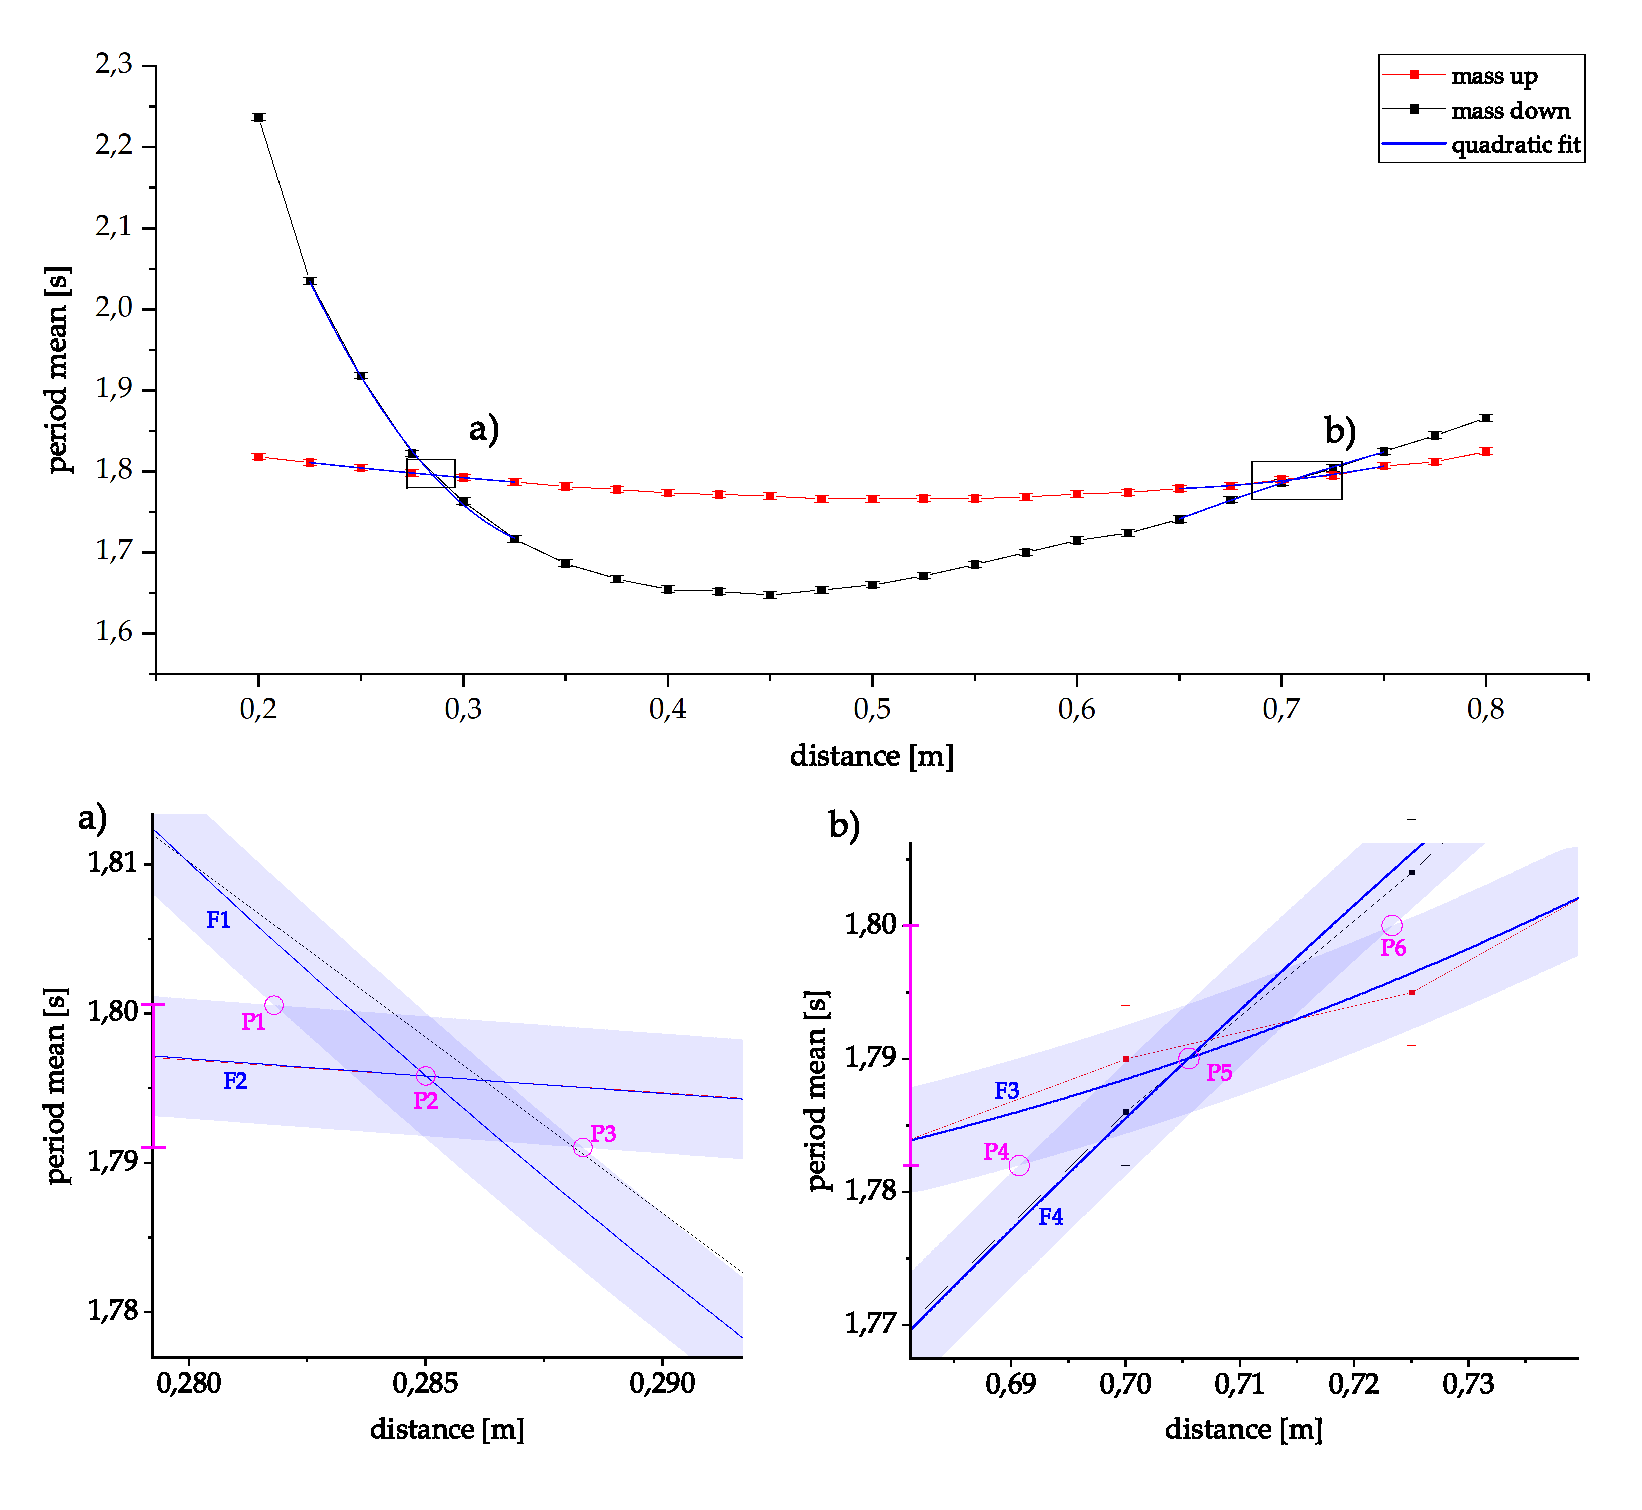
\includegraphics[width=450pt]{periodVsDistance.eps}
\caption{Periods of pendulum with fixed mass on the upper side (red) and lower side (black) for different mounting distances including detail view of intersection with quadratic fit and according uncertainties (blue)}
\end{figure}
\subsection{Evaluation}
If multiple measurements are available for a configuration, the arithmetic mean is used.
The five data points closest to the intersections are used for a quadratic fit, seen in blue in figure 2. From multiple measurements for one configuration of the pendulum, an error of $4$ms can be estimated, which is shown in light blue.
The resulting intersections show thee important points: P1 is the upper limit of the uncertainty, P2 is the point, where the quadratic fits intersect and P3 is the lower limit of the uncertainty.
These points are also seen for the second intersection.
We receive the data shown in table 1.
\begin{table}[hbt!]
\caption{Period for important points from figure 2}
\centering
\begin{tabular}{|c|c|}
\hline 
point & period [s] \\ 
\hline 
P1 & 1,8006 \\ 
\hline 
P2 & 1,7958 \\ 
\hline 
P3 & 1,7910 \\ 
\hline 
P4 & 1,7820 \\ 
\hline 
P5 & 1,7900 \\ 
\hline 
P6 & 1,8000 \\ 
\hline 
\end{tabular} 
\end{table}
The variance for points P2 and P5 are calculated by dividing the difference between the according minimum and maximum by 2.
The weighted mean gives a period of $1,7927(0,0057)$s.
Using equation 3, we obtain an acceleration of $9,827(0,030)\frac{\textrm{m}}{\textrm{s}^2}$.
\subsection{Discussion}
This result is close to an expected value of about $9,81\frac{\textrm{m}}{\textrm{s}^2}$. An exact value can hardly be found in literature since the acceleration is dependent on latitude, height and geological properties of the area where the measurement was performed.
Nevertheless, the value lies closer to a value, one might expect near the earth poles than in middle Europe.
\section{Coupled pendulum}
\subsection{Theory}
The coupled pendulum consists of two pendulum rods connected through a spring, with both pendulums exhibiting the same moment of inertia $J$ and oscillation period $\tau$.
\begin{figure}[hbt!]
\centering
\includegraphics[width=190pt]{coupled.png}
\caption{Important angles within the coupled pendulum in resting position (gray) and motion (black) \cite{1}.}
\end{figure}
After a few transformations using the small-angle approximation $\sin(\phi) \approx \phi$ the following differential equations emerge for the angular displacements of the two pendulums \cite{1}:
\begin{equation}
    \ddot{X} + \omega_{eq}^2 \cdot X = 0
\end{equation}
\begin{equation}
    \ddot{Y} + (\omega_{eq}^2 +2k^2) \cdot Y = 0,
\end{equation}
with $\omega_{eq}$ being the angular frequency of the two-part pendulum setup that has been deflected in the same direction. We also define $k$ as $k^2 := \frac{\kappa r^2}{J}$, with $\kappa$ being the spring constant and $a$ the distance between the spring and the suspension point of the pendulum.
We further assume the abbreviation $X:= \psi_1 + \psi_2$ and $Y:= \psi_1 - \psi_2$ , which are taken from the instructions \cite{1}. The solutions for equation 4 and 5 can be expressed by the following harmonic oscillations:
\begin{equation}
    X(t) = A_1 \cdot \sin(\omega_{eq}t) + A_2 \cdot \cos(\omega_{eq}t)
\end{equation}
\begin{equation}
    Y(t) = A_3 \cdot \sin(\omega_{opp}t) + A_4 \cdot \cos(\omega_{opp}t),
\end{equation}
with coefficients $A_1,A_2,A_3,A_4$ given by the initial angles and velocity of the two pendulums. 

\subsubsection{Equal deflection}
If the two pendulums are deflected in the same directions, meaning $\psi_1 = \psi_2$, the term $Y(t)$ goes zero and $X(t)$ is responsible for the oscillation. For the angular frequency of the pendulum in phase we get:
\begin{equation}
\omega_{eq} = \sqrt{\frac{mg \cdot l}{J}}
\end{equation}
\subsubsection{Opposite deflection}
If the pendulums are deflected in opposite directions, then $\psi_1 = - \psi_2$ and the angular frequency becomes
\begin{equation}
\omega_{opp} = \sqrt{\omega_{eq}^2 + 2k^2} = \sqrt{\frac{m \cdot g \cdot l + 2 \kappa r^2}{J}},
\end{equation}
which is greater than $\omega_{eq}$.
\subsubsection{Beat}
If only one of the two coupled pendulums is being deflected, a so-called beat develops, which is an interference pattern between two oscillations of slightly different frequencies, perceived as a periodic variation in amplitude whose rate is the difference of the two frequencies. 
After performing inverse transformations to the initial angles, the oscillation equations 3 and 4 can be solved by the following expressions:
\begin{equation}
 \psi_1 (t) = 2A \cdot \sin(\omega_M \cdot t)  \cdot \cos(\omega_B \cdot t) 
\end{equation}
\begin{equation}
 \psi_1 (t) = 2A \cdot \sin(\omega_M \cdot t)  \cdot \cos(\omega_B \cdot t).
\end{equation}
The mean angular frequency of the two pendulums is given by
\begin{equation}
    \omega_M = \frac{w_{eq}+w_{opp}}{2}
\end{equation}
and their amplitude is depended on the angular frequency of the beat:
\begin{equation}
        \omega_B = \frac{w_{opp}-w_{eq}}{2}.
\end{equation}
To compare the relative strength of the coupling, we define the coupling coefficient $K$:
\begin{equation}
    K = \frac{\omega_{opp}^2- \omega_{eq}^2}{\omega_{eq}^2 + \omega_{opp}^2} = \frac{\tau_{opp}^2- \tau_{eq}^2}{\tau_{eq}^2 + \tau_{opp}^2}.
\end{equation}
\begin{figure}[hbt!]
\centering
\includegraphics[width=300pt]{beat.png}
\caption{Example of a beat, where two oscillations with slightly different frequencies (orange and blue) constructively and destructively interfere to form a eye-shaped pattern (black) \cite{2}}
\end{figure}
\subsection{Experiment}
As shown in Figure 5, the coupled pendulum consists of two identical pendulum rods with four different holes each, in which a spring can be hung for coupling. If the rods, which have two needles as a suspension, are hung in the tip bearings provided in the bearing rod, the angular deflections of the pendulums can be measured via the magnetic sensors in the bearings.
\begin{figure}[hbt!]
\centering
\includegraphics[width=190pt]{coupled-theory.png}\caption{Coupled pendulum: a) bearing with protractor, b) pendulum rod with holes for spring, c) spring, d) adjustable weight. \cite{1}}
\end{figure}
At first, it is checked whether a phase difference occurs after a certain time when the pendulums are deflected in the same direction, which could falsify the later measurements. To do this, the pendulums, which are slightly deflected in the same direction, are allowed to swing freely for a few minutes without the spring attached, while the measurement data is recorded on the computer. We then evaluate whether the phase relationship between the two pendulums has changed noticeably over time. If this is the case, the masses on the pendulums are readjusted and the process is repeated. Otherwise one continues with the determination of the eigenmodes of the system. To do this, the pendulums, which are now coupled to a spring, are deflected in the same direction with roughly the same amplitude and allowed to oscillate for about a minute. After recording the data for about a minute, the process is repeated for a deflection in the opposite direction. Finally, measurements are carried out in which only one of the two pendulums is pushed in order to produce a beating. All three different variants of spring deflection are carried out for all four suspension holes and for both springs.
\subsection{Evaluation}
\paragraph{Oscillation periods of the eigenmodes}
For each series of measurements, the frequency spectrum was first evaluated with an FFT (Fast Fourier transform) in order to determine the extent of hidden coupling and to get the main frequencies of the signal analytically.
We then determined the angular frequencies $\omega_{eq}$ and $\omega_{opp}$ by performing a linear fit and calculated their period durations $\tau_{opp}$ and $\tau_{eq}$ with the following relationships:
\begin{equation}
    \tau = \frac{2\pi}{\omega}.
\end{equation}
\paragraph{Beat}
Following that, one can determine the mean angular frequency and the beat frequency through the following relationship:
\begin{equation}
    \omega_{b,theo} = \frac{\omega_{opp -\omega_{eq}}}{2},
\end{equation}
\begin{equation}
    \omega_{m,theo} = \frac{\omega_{opp +\omega_{eq}}}{2}.
\end{equation}
Results for this are shown in Figure 6.
\begin{figure}[hbt!]
\centering
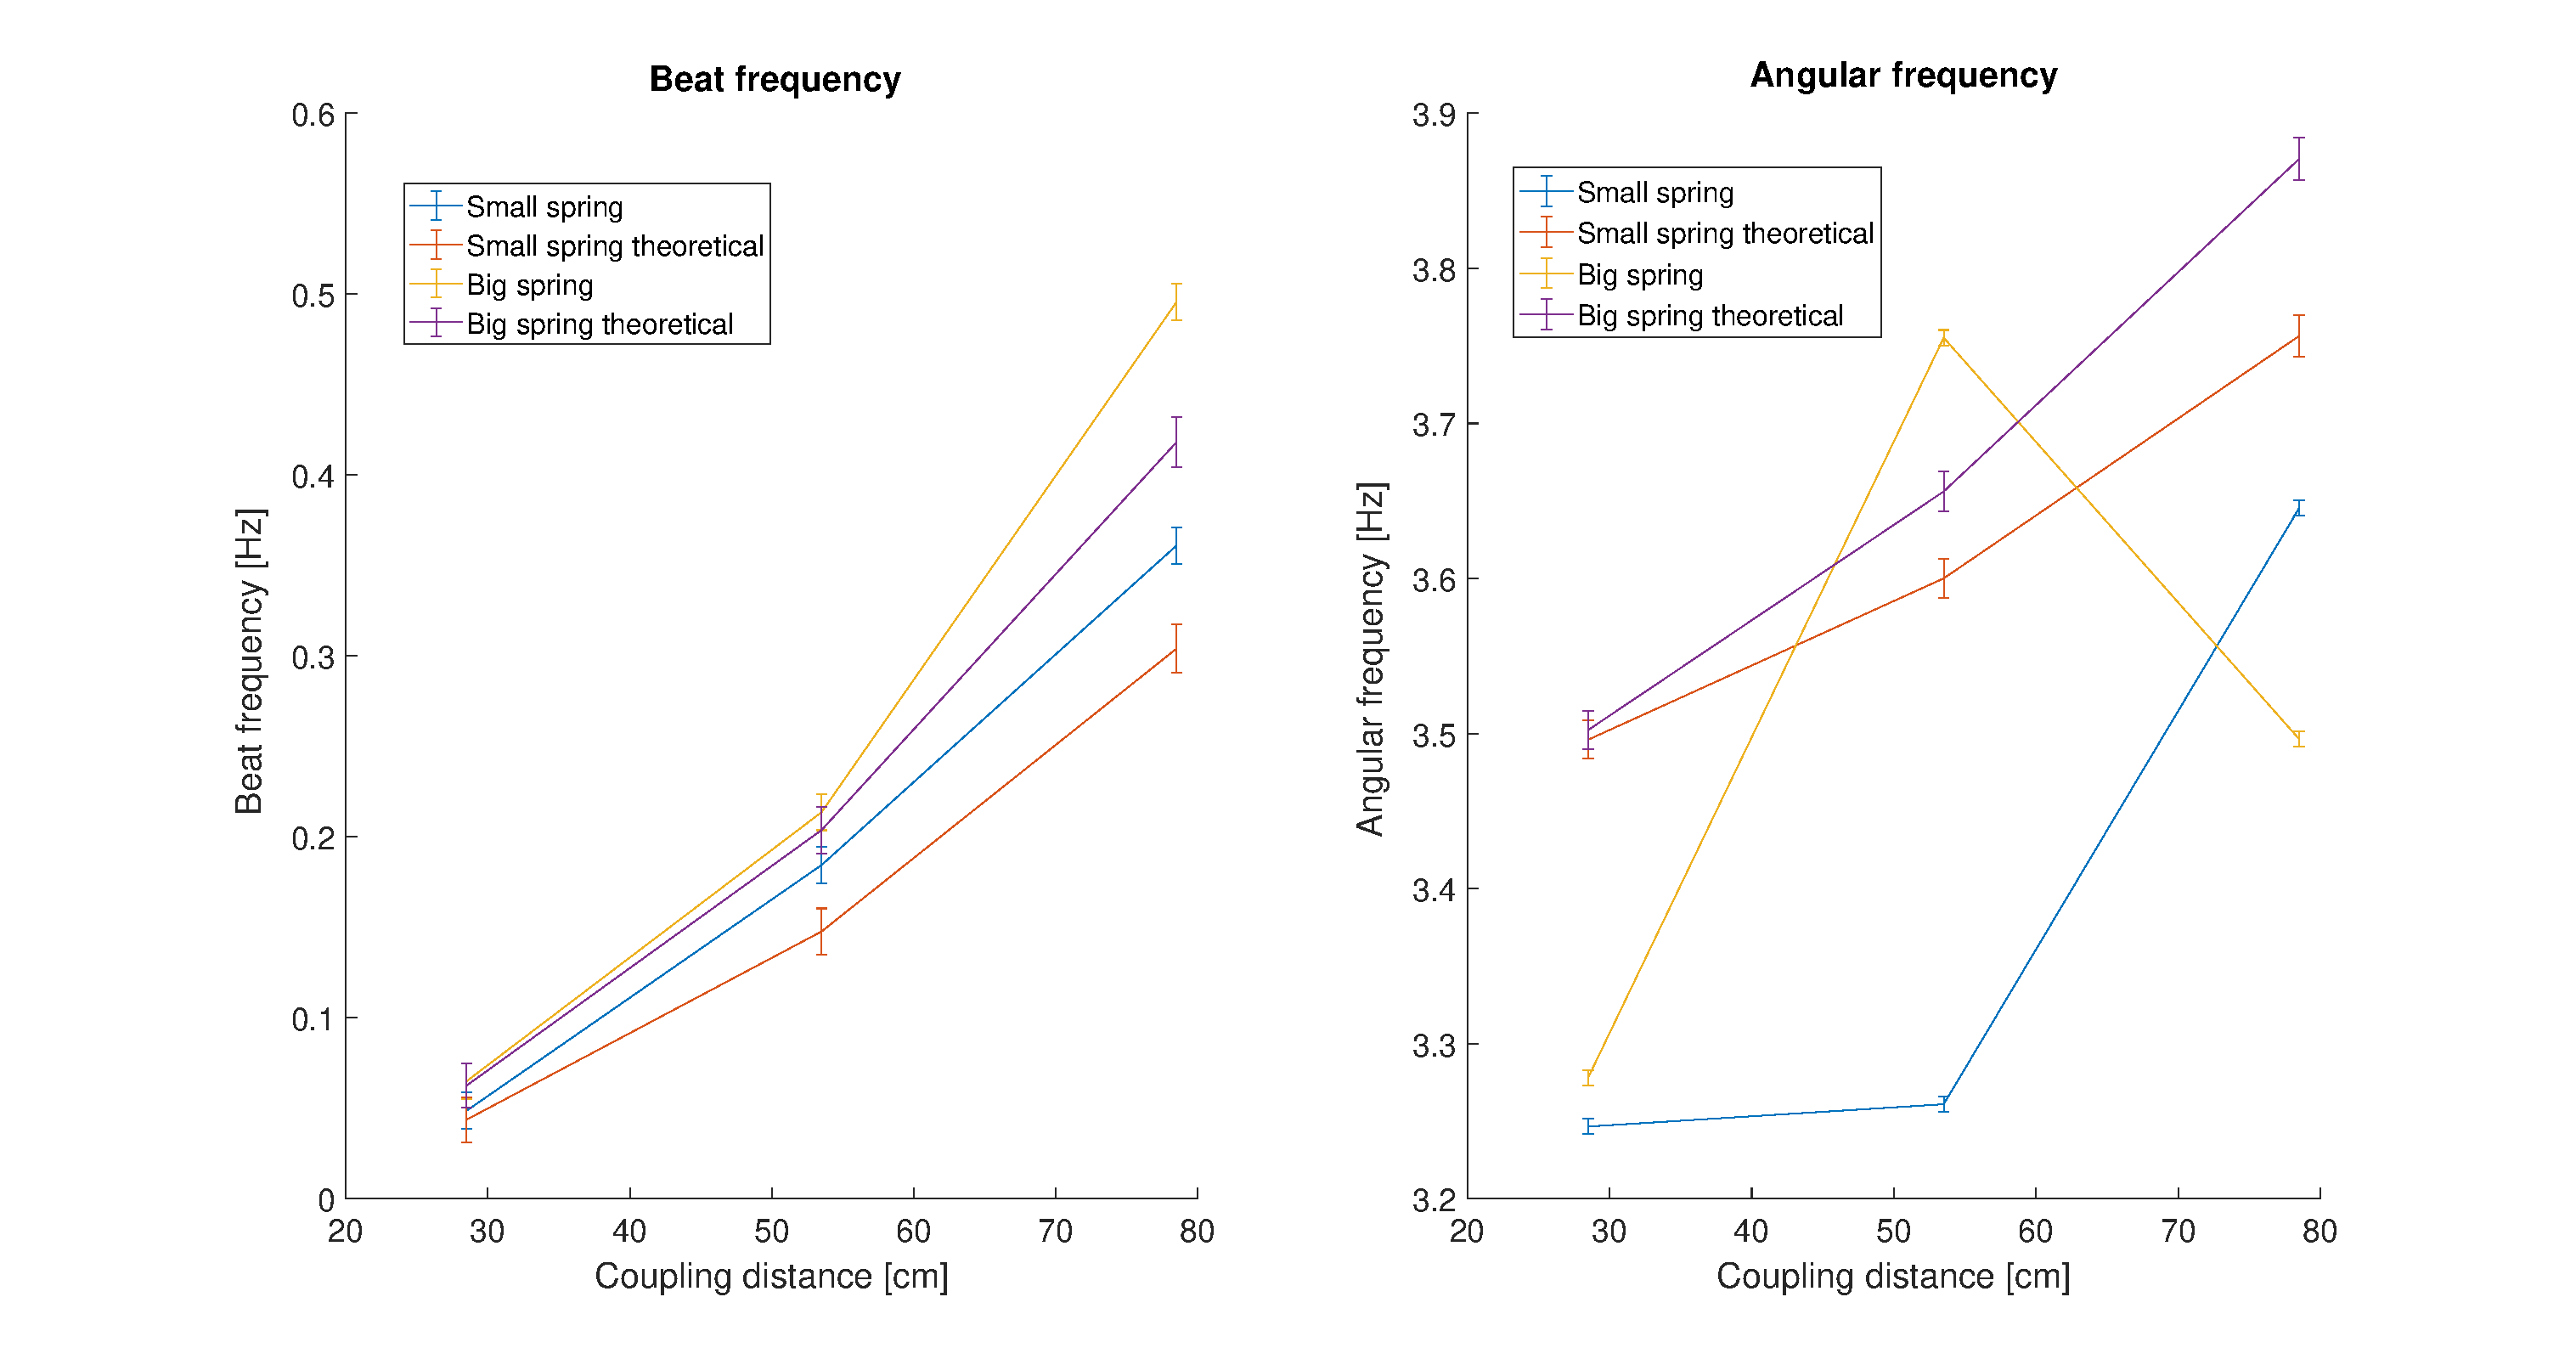
\includegraphics[width=480pt]{beat-vs-ang-coupled.eps}
\caption{Beat frequency vs Angular frequency of each coupling distance}
\end{figure}
\begin{figure}[hbt!]
\centering
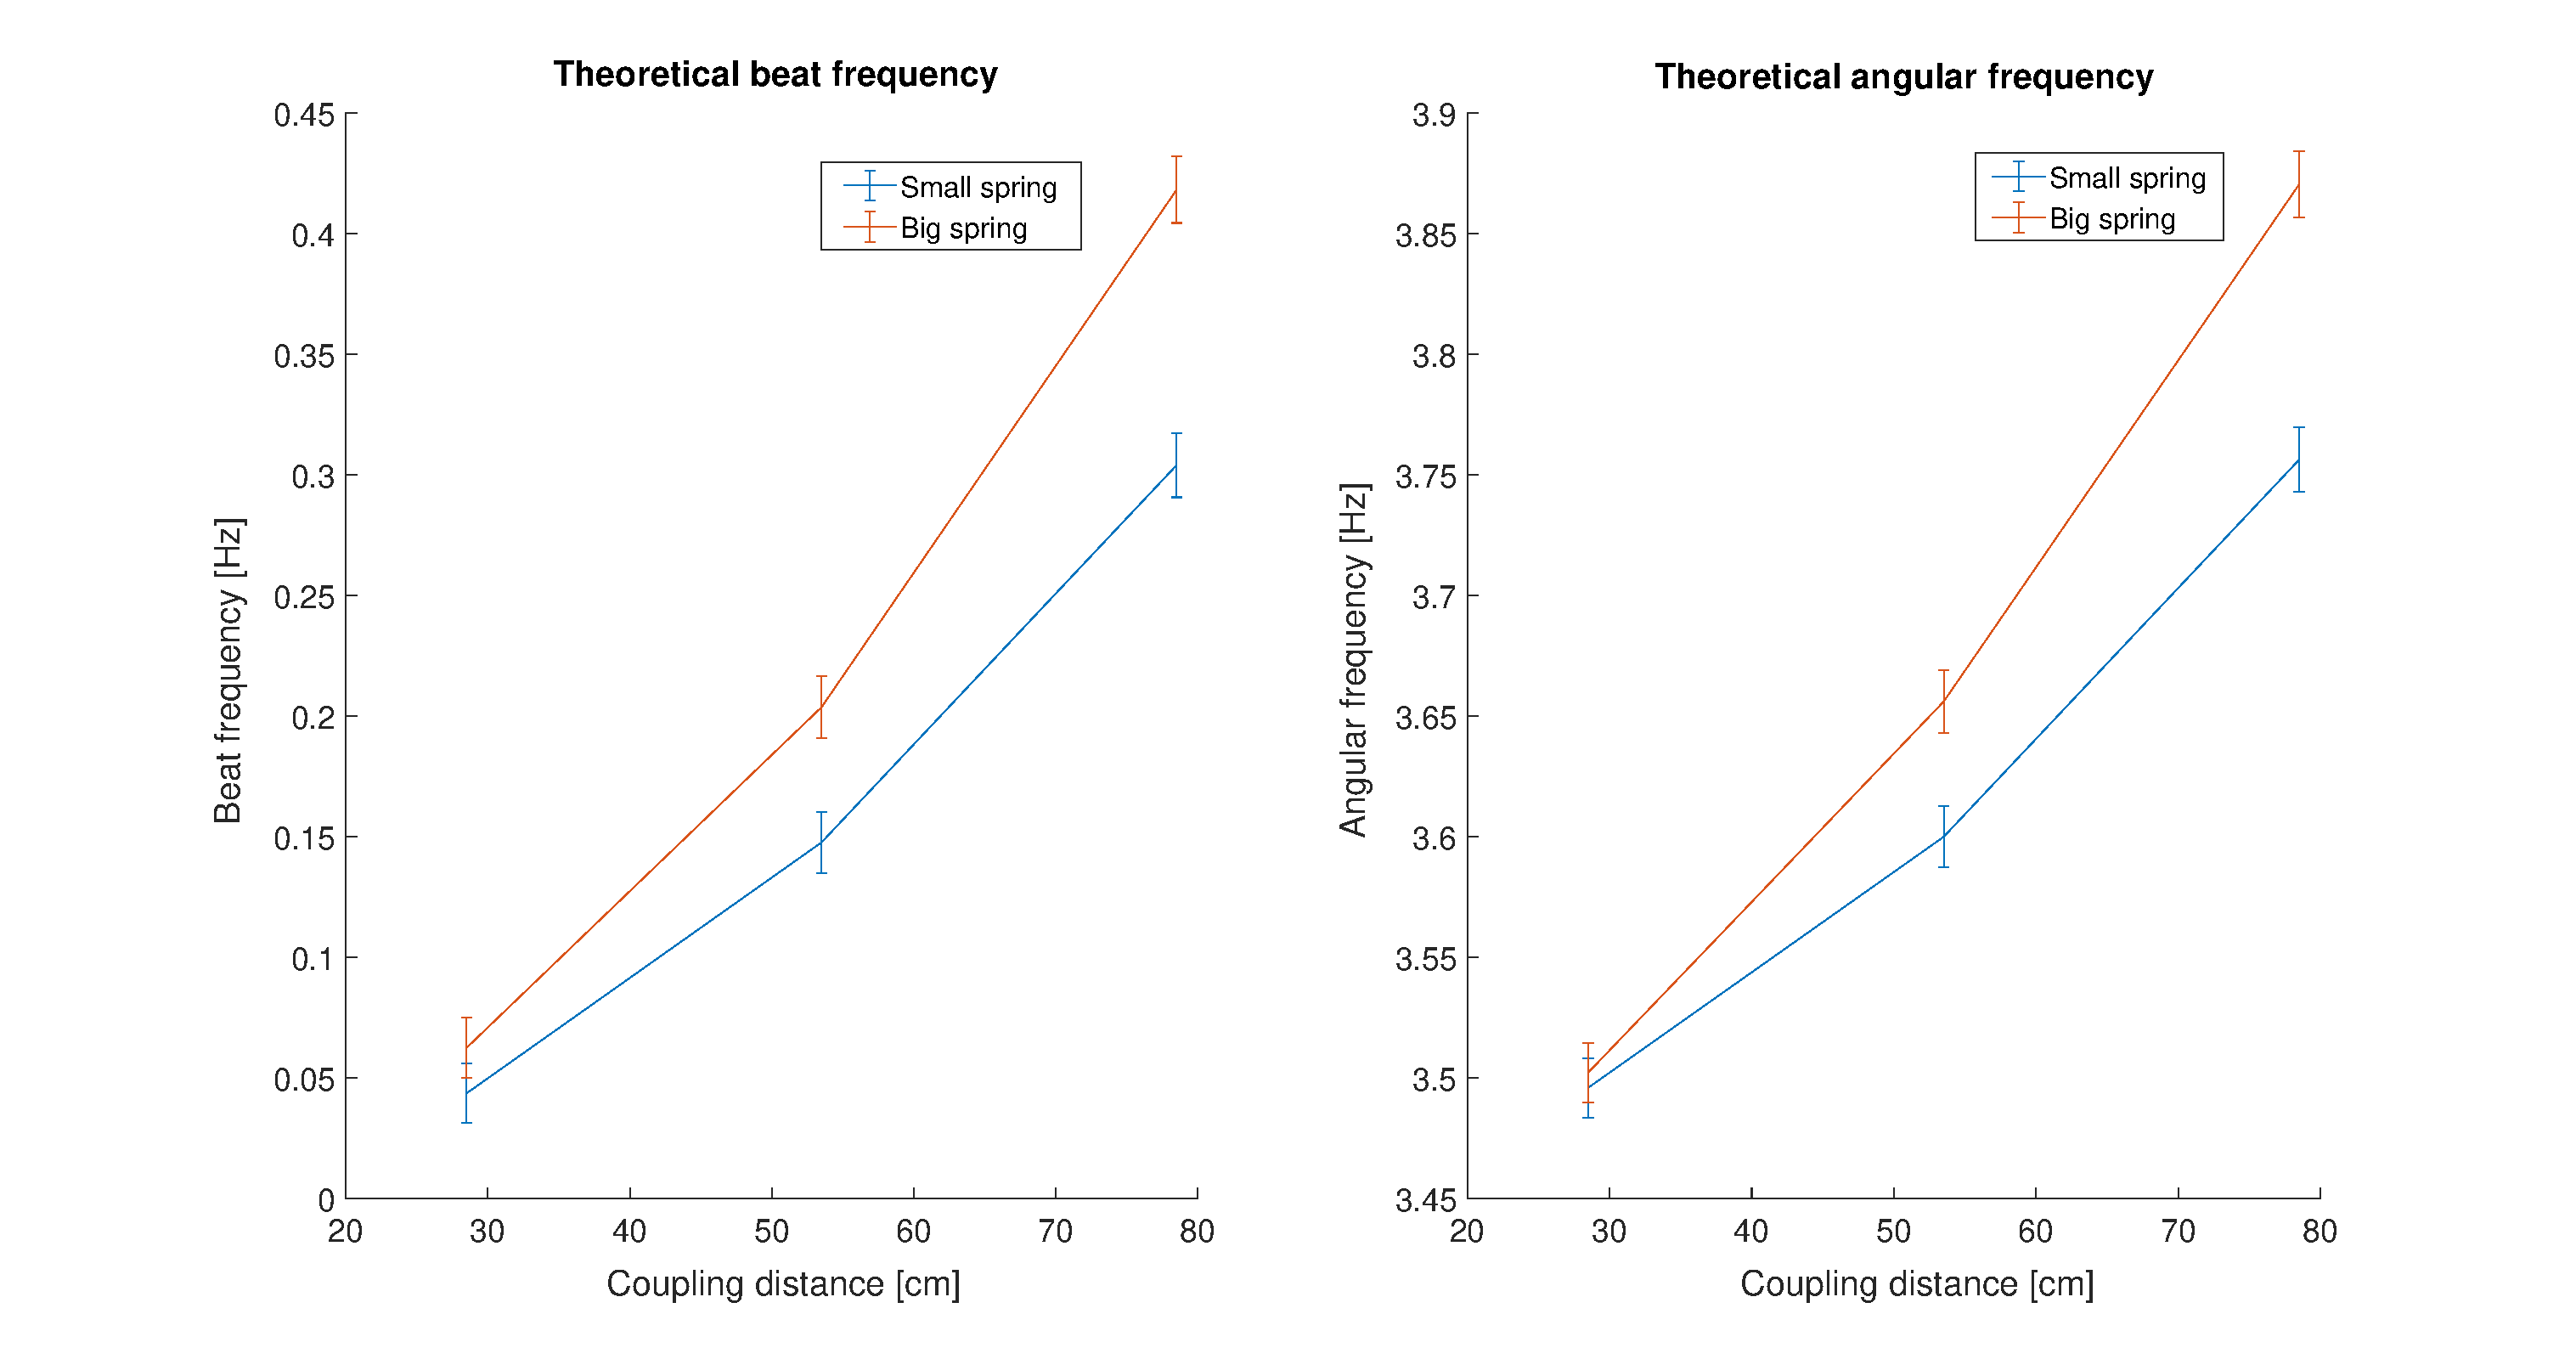
\includegraphics[width=480pt]{theoretical.eps}
\caption{Standalone graph showcasing both theoretical calculation in detail}
\end{figure}

One might observe a significant anomaly at the second coupling distance of $53.5$ cm, that most likely occurred through an imperfect deflection of one of the pendulums.
If we plot the two oscillations of the pendulums and their beat, or just by looking at the raw data, we can also see that the first pendulum has a much higher amplitude as the second one (Figure 8). 
\begin{figure}[hbt!]
\centering
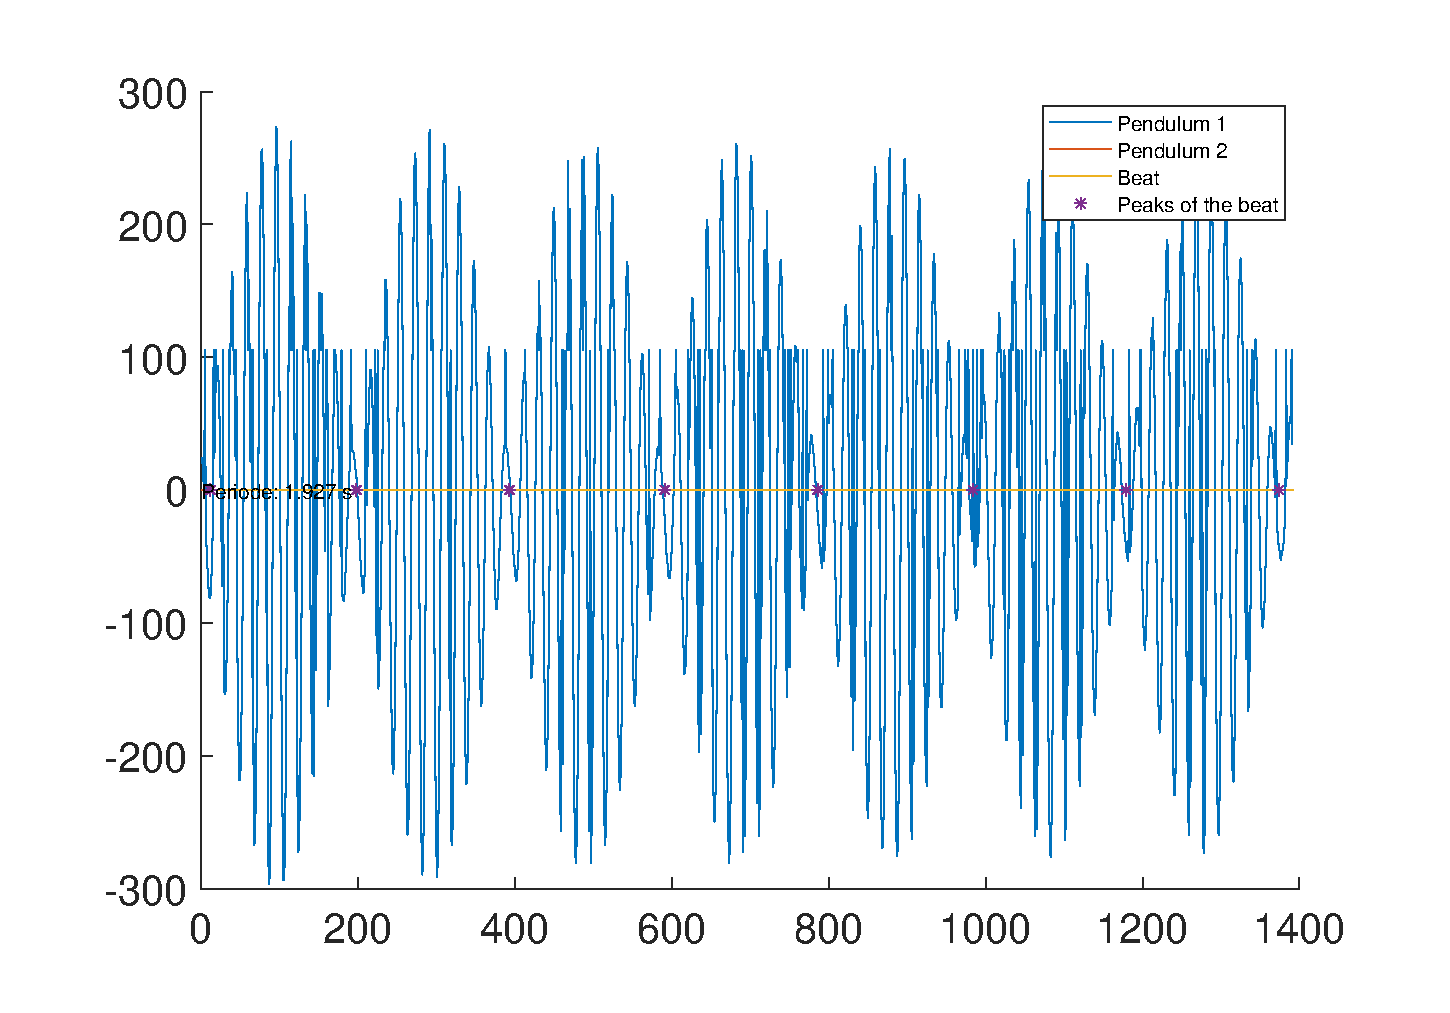
\includegraphics[width=400pt]{precision.eps}
\caption{Snapshot showcasing the difference between oscillations and the beat of the pendulums}
\end{figure}
Because of this our precision for the second pendulum is much lower as for the first one. Zooming in to the plot, you can observe that the significance of the second pendulums values only lie in the second decimal place and are therefore less accurate. We tried solving this issue while performing the experiment, but after a while of troubleshooting we were told that the setup was sufficient.
\begin{figure}[hbt!]
\centering
\includegraphics[width=400pt]{closeup.eps}
\caption{Close up view of the second oscillation}
\end{figure}
\paragraph{Coupling coefficient}
Finally, the coupling coefficient of the springs is determined as a function of the coupling distance r, by using the aforementioned equation 14. The coupling coefficients obtained in this way are shown in Figure 10. Looking at the values, one finds that the theoretical and experimental values differ more as the coupling distance increases.
\begin{figure}[hbt!]
\centering
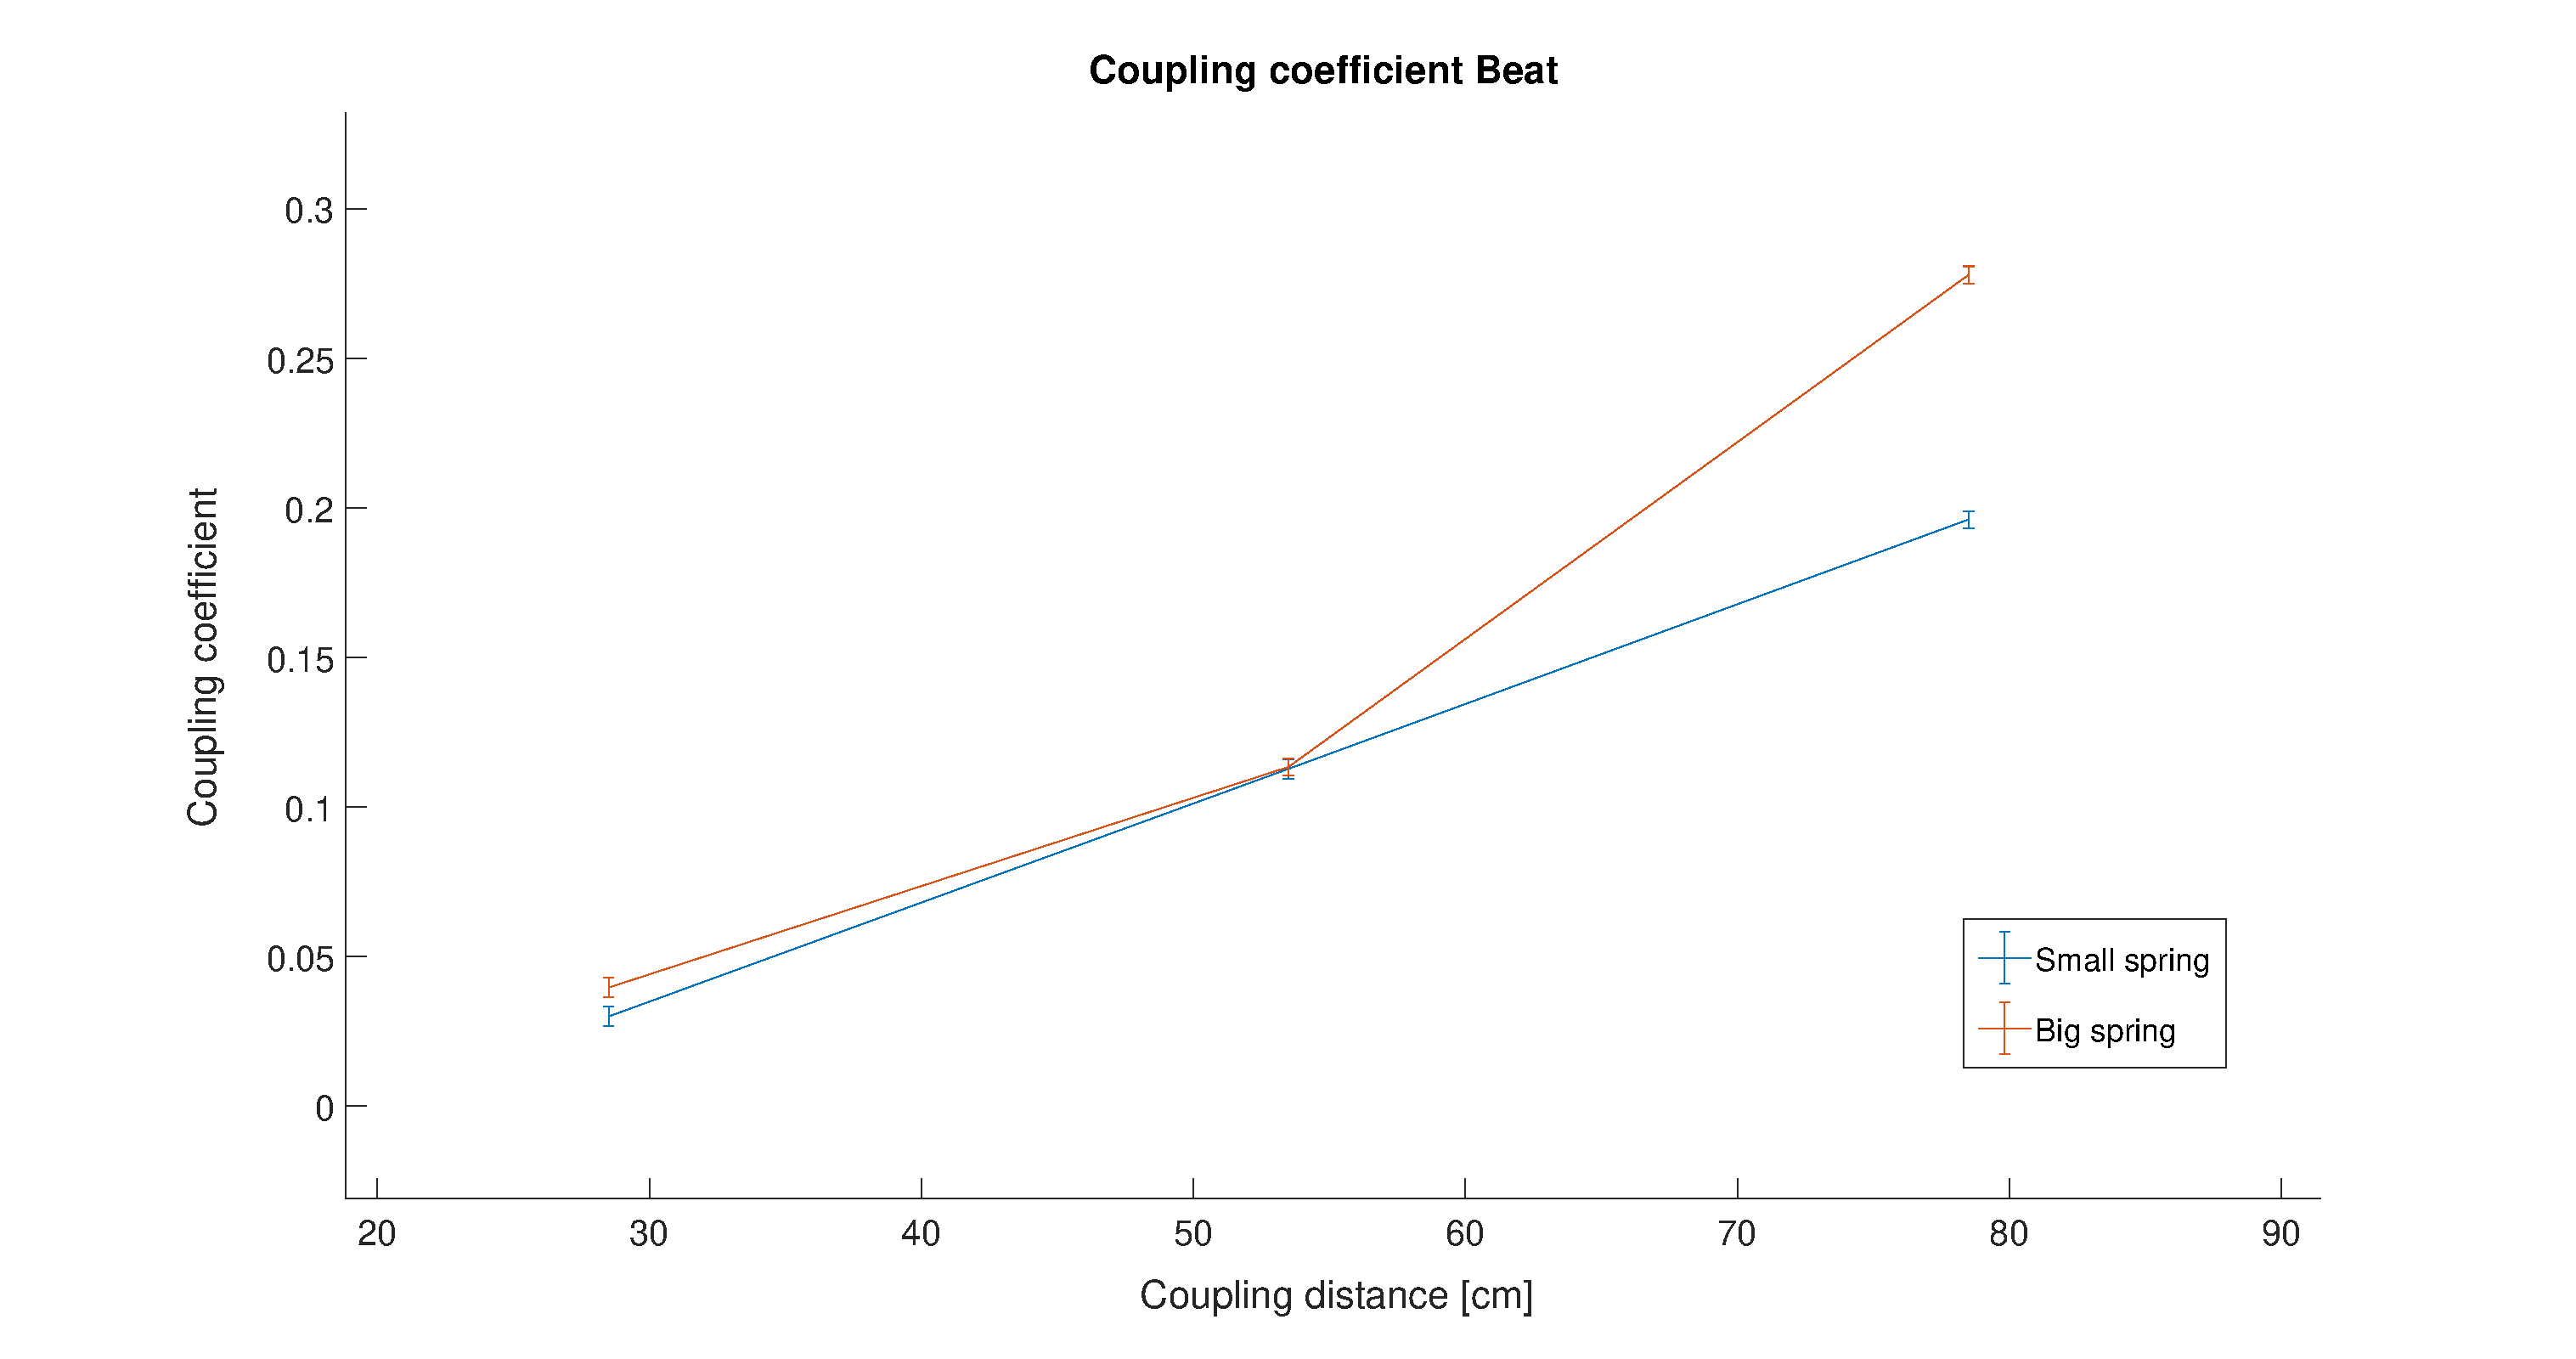
\includegraphics[width=480pt]{coupling-coffefficient-vs-distance.eps}
\caption{Coupling coefficient vs coupling distance}
\end{figure}






\subsection{Discussion}
Our results for the coupled pendulum lie barely close enough to the theoretical values so that we still can call our calculations representative of what actually happened. Although our predictions could be vastly improved by remeasuring the values for the aforementioned anomaly at coupling distance two (Figure 6b). We also observed, while performing the experiment, that there is quite a lot of play in the outwards and inwards motion of the two pendulums, which could lead to non negligible errors.
\section{References}
\begin{thebibliography}{9}
\bibitem{1}
Fakultät für Physik. \emph{Pendel (PEN)}. Technische Universität München. 31.05.2022.
\textbf{URL:} \url{https://www.ph.tum.de/academics/org/labs/ap/ap1/PEN.pdf}.


\bibitem{2}
Beat figure. \emph{Lesson Worksheet: Beat Frequencies.
} Nagwa Limited. 12.06.2022.
\textbf{URL:} \url{https://images.nagwa.com/figures/353178374706/1.svg}.





\end{thebibliography}
\section{Appendix}
\subsection{Error estimation}
\paragraph{Reversed pendulum}
For the experiment of the reversed pendulum, two sources of errors have to be considered: the distance between the axes and the timing of one period.
The distance between the axes was exactly 80,0cm, measuring with a ruler. Due to manufacturing error of the ruler, we estimate an uncertainty of 1mm.
For the period, the photoelectric sensors uncertainty of 1ms has to be added to an estimated uncertainty based on differences between measurements with the same configuration of 4ms.
\begin{equation}
\sqrt{(1\textrm{ms})^2+(4\textrm{ms})^2} \approx 4 \textrm{ms}
\end{equation}
This error is plotted in figure 2 and used to graphically determine an upper and lower limit of uncertainty.
As already mentioned, the difference between upper and lower limit are used to calculate a weighted mean using
\begin{equation}
\tau_{mean} = \frac{\frac{1}{u(\tau_1)^2} \cdot \tau_{1} + \frac{1}{u(\tau_2)^2} \cdot \tau_2}{\frac{1}{u(\tau_1)^2} + \frac{1}{u(\tau_2)^2}}
\end{equation}
and the according uncertainties
\begin{equation}
u(\tau_{mean}) = max(u_{int}(\tau_{mean}), u_{ext}(\tau_{mean})).
\end{equation}
\begin{equation}
u_{int}(\tau_{mean}) = \sqrt{\frac{1}{\frac{1}{u(\tau_1)^2}+\frac{1}{u(\tau_2)^2}}}
\end{equation}
\begin{equation}
u_{ext}(\tau_{mean}) = \sqrt{\frac{\frac{1}{u(\tau_1)^2} \cdot (\tau_{mean} - \tau_1)^2+ \frac{1}{u(\tau_2)^2} \cdot (\tau_{mean} - \tau_2)^2}{(2-1)\cdot (\frac{1}{u(\tau_1)^2}+\frac{1}{u(\tau_2)^2})}}
\end{equation}
The uncertainty of equation 3 is given by
\begin{equation}
u(g) = \sqrt{\frac{\delta g}{\delta L}^2 \cdot u(L)^2 + \frac{\delta g}{\delta\tau}^2 \cdot u(\tau_{mean})^2} = \sqrt{\frac{4\pi^2}{\tau^2}^2 \cdot u(L)^2 + \frac{8\pi^2L}{\tau^3}^2 \cdot u(\tau_{mean})^2}
\end{equation}
An other factor that may influence the results is the small-angle approximation which was used to simplify the differential equation for the pendulum.
All measurements were performed with an angle of $\leq 5°$, therefore the resulting deviation should be very small ($\leq 0,13\% $) and is not considered any further. 

\paragraph{Coupled pendulum}
For the experiment with the coupled pendulums, mainly one source of error has to be considered, which is the timing of the periods. We can safely neglected the error of the magnetic probe which measures the deflections and the length of the rods, as they both tend to very small. With a resolution of 0.1s and a period interval of about $1.5\rightarrow 2$s , there is at least a basic inaccuracy of $5\%$. In addition, oscillations that are not optimally deflected lead to small beats even in the case of simple deflections in equal and opposite directions, so that the inaccuracy from measurement series to measurement series must be estimated together with the human-related reading accuracy at the respective discretion. Thus there is no closed expression for the uncertainty of $\omega$:
\begin{equation}
u(\omega)= \frac{u(\tau)}{\tau}.
\end{equation}
For any theoretical values of $\omega_M$ and $\omega_B$, which are calculated from $\omega_{eq}$ and $\omega_{opp}$, we get an error of:
\begin{equation}
u(\omega_{M,B})= \frac{1}{2} \sqrt{\omega_{opp}^2+ \omega_{eq}^2}
\end{equation}
and
\begin{equation}
u(\omega_{opp,eq})= \frac{1}{2} \sqrt{\omega_{M}^2+ \omega_{B}^2}.
\end{equation}
For the error propagation of the coupling coefficient we get:
\begin{equation}
u(K)= \frac{4 \omega_{opp}\omega_{eq}}{(\omega_{opp}^2+\omega_{eq}^2)^2} \cdot \sqrt{(\omega_{eq} \cdot u(\omega_{opp})^2 + (\omega_{opp} \cdot u(\omega_{eq})^2}.
\end{equation}


\subsection{Lab notebook}

\begin{figure*}[tb] 
\centering
 \makebox[\textwidth]{\includegraphics[width=.8\paperwidth]{lab1.jpeg}}
\end{figure*}

\begin{figure*}[tb] 
\centering
 \makebox[\textwidth]{\includegraphics[width=.8\paperwidth]{lab2.jpeg}}
\end{figure*}

\begin{figure*}[tb] 
\centering
 \makebox[\textwidth]{\includegraphics[width=.8\paperwidth]{lab3.jpeg}}
\end{figure*}

\end{document}
